

%% AAPT Physics Olympiad F=ma Questions
%%----------------------------------------


%% this section contains 50 problems


%% PhysicsOlympiad 2015
%%----------------------------------------
\element{aapt}{ %% Olympiad-A3
\begin{question}{Olympiad-2015-Q04}
    A \SI{2.0}{\kilo\gram} box is originally at rest on a horizontal surface
        where the coefficient of static friction between the box and the surface
        is $\mu_s$ and the coefficient of the kinetic friction between the box
        and the surface is $\mu_k=\num{0.90}\mu_s$.
    An external horizontal force of magnitude $P$ is then applied to the box.
    Which of the following is a graph of the acceleration of the box a versus the external force $P$?
    \begin{multicols}{2}
    \begin{choices}
        \AMCboxDimensions{down=-1.5em}
        %% ANS is A
        \correctchoice{
            \begin{tikzpicture}
                \begin{axis}[
                    axis y line=left,
                    axis x line=bottom,
                    axis line style={->},
                    xlabel={Force $P$},
                    xtick=\empty,
                    ylabel={acceleration $a$},
                    ytick=\empty,
                    xmin=0,xmax=11,
                    ymin=0,ymax=11,
                    width=0.95\columnwidth,
                    very thin,
                ]
                \addplot[line width=1pt,mark=\empty] plot coordinates {(0,0) (3,0) (3,1) (10,8)};
                \end{axis}
            \end{tikzpicture}
        }
        \wrongchoice{
            \begin{tikzpicture}
                \begin{axis}[
                    axis y line=left,
                    axis x line=bottom,
                    axis line style={->},
                    xlabel={Force $P$},
                    xtick=\empty,
                    ylabel={acceleration $a$},
                    ytick=\empty,
                    xmin=0,xmax=11,
                    ymin=0,ymax=11,
                    width=0.95\columnwidth,
                    very thin,
                ]
                \addplot[line width=1pt,mark=\empty] plot coordinates {(0,0) (3,0) (3,3) (10,10)};
                \end{axis}
            \end{tikzpicture}
        }
        \wrongchoice{
            \begin{tikzpicture}
                \begin{axis}[
                    axis y line=left,
                    axis x line=bottom,
                    axis line style={->},
                    xlabel={Force $P$},
                    xtick=\empty,
                    ylabel={acceleration $a$},
                    ytick=\empty,
                    xmin=0,xmax=11,
                    ymin=0,ymax=11,
                    width=0.95\columnwidth,
                    very thin,
                ]
                \addplot[line width=1pt,mark=\empty] plot coordinates {(0,0) (3,0) (10,7)};
                \end{axis}
            \end{tikzpicture}
        }
        \wrongchoice{
            \begin{tikzpicture}
                \begin{axis}[
                    axis y line=left,
                    axis x line=bottom,
                    axis line style={->},
                    xlabel={Force $P$},
                    xtick=\empty,
                    ylabel={acceleration $a$},
                    ytick=\empty,
                    xmin=0,xmax=11,
                    ymin=0,ymax=11,
                    width=0.95\columnwidth,
                    very thin,
                ]
                \addplot[line width=1pt,mark=\empty] plot coordinates {(0,3) (1,3) (8,11)};
                \end{axis}
            \end{tikzpicture}
        }
        \wrongchoice{
            \begin{tikzpicture}
                \begin{axis}[
                    axis y line=left,
                    axis x line=bottom,
                    axis line style={->},
                    xlabel={Force $P$},
                    xtick=\empty,
                    ylabel={acceleration $a$},
                    ytick=\empty,
                    xmin=0,xmax=11,
                    ymin=0,ymax=11,
                    width=0.95\columnwidth,
                    very thin,
                ]
                \addplot[line width=1pt,mark=\empty] plot coordinates {(0,0) (3,3) (3,4) (9,10)};
                \end{axis}
            \end{tikzpicture}
        }
    \end{choices}
    \end{multicols}
\end{question}
}


%% PhysicsOlympiad 2014
%%----------------------------------------
\element{aapt}{ %% Olympiad-A3
\begin{question}{Olympiad-2014-Q02}
    A ball rolls without slipping down an inclined plane as shown in the diagram.
    Which of the following vectors best represents the direction of the total
        force that the ball exerts on the plane?
    \begin{center}
    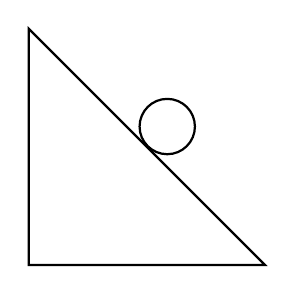
\begin{tikzpicture}
        %% NOTE: 45 degree slope
        \draw[thick] (0,0) -- (3,0) -- (0,3) -- cycle;
        \node[thick,draw,circle,minimum size=2em,anchor=south west] at (1.5,1.5) {};
    \end{tikzpicture}
    \end{center}
    \begin{multicols}{2}
    \begin{choices}
        \AMCboxDimensions{down=-0.85cm}
        \wrongchoice{
            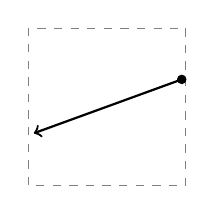
\begin{tikzpicture}
                \draw[dashed,draw=white!50!black] (+0.05,+0.65) rectangle (-1.95,-1.35);
                \draw[fill] (0,0) circle (1.5pt);
                \draw[thick,->] (0,0) -- (200:2.0cm);
            \end{tikzpicture}
        }
        \wrongchoice{
            \begin{tikzpicture}
                \draw[dashed,draw=white!50!black] (-2.00,-1.00) rectangle (0.0,+1.0);
                \draw[fill] (0,0) circle (1.5pt);
                \draw[thick,->] (0,0) -- (180:2.0cm);
            \end{tikzpicture}
        }
        \wrongchoice{
            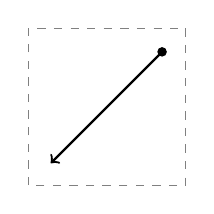
\begin{tikzpicture}
                \draw[dashed,draw=white!50!black] (+0.3,+0.3) rectangle (-1.7,-1.7);
                \draw[fill] (0,0) circle (1.5pt);
                \draw[thick,->] (0,0) -- (225:2.0cm);
            \end{tikzpicture}
        }
        \wrongchoice{
            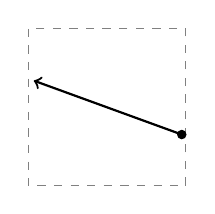
\begin{tikzpicture}
                \draw[dashed,draw=white!50!black] (+0.05,-0.65) rectangle (-1.95,+1.35);
                %\draw[dashed,draw=white!50!black] (-1.00,0.00) rectangle (+1.0,-2.0);
                \draw[fill] (0,0) circle (1.5pt);
                \draw[thick,->] (0,0) -- (160:2.0cm);
            \end{tikzpicture}
        }
        %% NOTE: ans is E
        %% The arrow is straight down in the case of 45 deg
        \correctchoice{
            \begin{tikzpicture}
                \draw[dashed,draw=white!50!black] (-1.00,-0.00) rectangle (+1.0,-2.0);
                \draw[fill] (0,0) circle (1.5pt);
                \draw[thick,->] (0,0) -- (270:2.0cm);
            \end{tikzpicture}
        }
    \end{choices}
    \end{multicols}
\end{question}
}

\element{aapt}{ %% Olympiad-A3
\begin{question}{Olympiad-2014-Q09}
    A \SI{5.0}{\kilo\gram} object undergoes a time-varying force as shown in the graph below.
    \begin{center}
    \begin{tikzpicture}
        \begin{axis}[
            axis y line=left,
            axis x line=bottom,
            axis line style={->},
            xlabel={time},
            x unit=\si{\second},
            xtick={0,1,2,3,4,5,6,7,8},
            minor x tick num=1,
            ylabel={force},
            y unit=\si{\newton},
            ytick={0,1,2,3,4},
            minor x tick num=1,
            grid=major,
            xmin=0,xmax=8.1,
            ymin=0,ymax=4.1,
            width=0.8\columnwidth,
            height=0.5\columnwidth,
        ]
        \addplot[line width=1pt,mark=\empty] plot coordinates { (0,0) (3,3) (7,1) (8,1) };
        \end{axis}
    \end{tikzpicture}
    \end{center}
    If the velocity at $t=\SI{0.0}{\second}$ is \SI[retain-explicit-plus]{+1.0}{\meter\per\second},
        what is the velocity of the object at $t=\SI{7}{\second}$?
    \begin{multicols}{2}
    \begin{choices}
        \wrongchoice{\SI{2.45}{\meter\per\second}}
        \wrongchoice{\SI{2.50}{\meter\per\second}}
      \correctchoice{\SI{3.50}{\meter\per\second}}
        \wrongchoice{\SI{12.5}{\meter\per\second}}
        \wrongchoice{\SI{15.0}{\meter\per\second}}
    \end{choices}
    \end{multicols}
\end{question}
}

\element{aapt}{ %% Olympiad-A3
\begin{question}{Olympiad-2014-Q18}
    Consider the following diagram of a box and two weight scales.
    Scale $A$ supports the box via a massless rope.
    A pulley is attached to the top of the box;
        a second massless rope passes over the pulley,
        one end is attached to the box and the other end to scale $B$.
    The two scales read indicate the tensions $T_A$ and $T_B$ in the ropes.
    Originally scale $A$ reads \SI{30}{\newton} and scale $B$ reads \SI{20}{\newton}.
    \begin{center}
        %% NOTE: tikz?
        \includegraphics[keepaspectratio,scale=0.6]{Olympiad2014-Q18}
    \end{center}
    If an additional force pulls down on scale $B$ so that the reading increases to
        \SI{30}{\newton}, what will be the new reading on scale $A$?
    \begin{multicols}{3}
    \begin{choices}
        \wrongchoice{\SI{35}{\newton}}
      \correctchoice{\SI{40}{\newton}}
        \wrongchoice{\SI{45}{\newton}}
        \wrongchoice{\SI{50}{\newton}}
        \wrongchoice{\SI{60}{\newton}}
    \end{choices}
    \end{multicols}
\end{question}
}

\element{aapt}{ %% Olympiad-A3
\begin{question}{Olympiad-2014-Q19}
    A helicopter is flying horizontally at constant speed.
    A perfectly flexible uniform cable is suspended beneath the helicopter;
        air friction on the cable is not negligible.
    %% Begin Question
    Which of the following diagrams best shows the shape of the cable
        as the helicopter flies through the air to the right?
    \begin{multicols}{2}
    \begin{choices}
        %% NOTE: tikz?
        \AMCboxDimensions{down=-2cm}
        \wrongchoice{\includegraphics[keepaspectratio,scale=1.0]{Olympiad2014-Q19-A}}
      \correctchoice{\includegraphics[keepaspectratio,scale=1.0]{Olympiad2014-Q19-B}}
        \wrongchoice{\includegraphics[keepaspectratio,scale=1.0]{Olympiad2014-Q19-C}}
        \wrongchoice{\includegraphics[keepaspectratio,scale=1.0]{Olympiad2014-Q19-D}}
        \wrongchoice{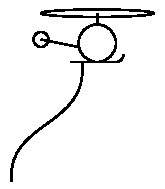
\includegraphics[keepaspectratio,scale=1.0]{Olympiad2014-Q19-E}}
    \end{choices}
    \end{multicols}
\end{question}
}


%% PhysicsOlympiad 2013
%%----------------------------------------
\newcommand{\myOlympiadThirteenQzeroFive}{
\begin{tikzpicture}
    \begin{axis}[
        axis y line=left,
        axis x line=bottom,
        axis line style={->},
        xlabel={time},
        x unit=\si{\second},
        xtick={0,2,4,6,8,10,12,14,16,18,20,22,24,26},
        ylabel={scale reading},
        y unit=\si{\kilo\gram},
        ytick={0,20,40,60,80,100,120},
        %grid=major,
        xmin=0,xmax=26,
        ymin=0,ymax=120,
        width=0.90\columnwidth,
        height=0.45\columnwidth,
    ]
    \addplot[mark=\empty] plot coordinates { (0,80) (2,80) (2,60) (4,60) (4,80) (22,80) (22,100) (24,100) (24,80) (26,80) };
    \end{axis}
\end{tikzpicture}
}

\element{aapt}{ %% Olympiad-A3
\begin{question}{Olympiad-2013-Q05}
    A student steps onto a stationary elevator and stands on a bathroom scale.
    The elevator then travels from the top of the building to the bottom.
    The student records the reading on the scale as a function of time.
    \begin{center}
        \myOlympiadThirteenQzeroFive
    \end{center}
    At what time(s) does the student have maximum downward velocity?
    \begin{choices}
        \wrongchoice{At all times between \SI{2}{\second} and \SI{4}{\second}}
        \wrongchoice{At \SI{4}{\second} only}
      \correctchoice{At all times between \SI{4}{\second} and \SI{22}{\second}}
        \wrongchoice{At \SI{22}{\second} only}
        \wrongchoice{At all times between \SI{22}{\second} and \SI{24}{\second}}
    \end{choices}
\end{question}
}

\element{aapt}{ %% Olympiad-A3
\begin{question}{Olympiad-2013-Q06}
    A student steps onto a stationary elevator and stands on a bathroom scale.
    The elevator then travels from the top of the building to the bottom.
    The student records the reading on the scale as a function of time.
    \begin{center}
        \myOlympiadThirteenQzeroFive
    \end{center}
    How tall is the building?
    \begin{multicols}{3}
    \begin{choices}
        \wrongchoice{\SI{50}{\meter}}
        \wrongchoice{\SI{80}{\meter}}
      \correctchoice{\SI{100}{\meter}}
        \wrongchoice{\SI{150}{\meter}}
        \wrongchoice{\SI{400}{\meter}}
    \end{choices}
    \end{multicols}
\end{question}
}

\element{aapt}{ %% Olympiad-A3
\begin{question}{Olympiad-2013-Q11}
    A right-triangular wooden block of mass $M$ is at rest on a table, as shown in figure.
    Two smaller wooden cubes, both with mass $m$,
        initially rest on the two sides of the larger block.
    As all contact surfaces are frictionless,
        the smaller cubes start sliding down the larger block while the block remains at rest.
    What is the normal force from the system to the table?
    \begin{center}
    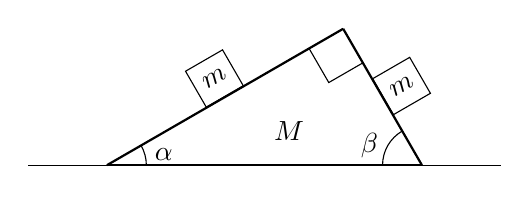
\begin{tikzpicture}
        %% Triangle
        \draw (-3,0) -- (3,0);
        \draw[thick] (-2,0) -- (2,0);
        \draw[thick] (-2,0) -- ++(30:3.464);
        \draw[thick] (+2,0) -- ++(120:2);
        \node[anchor=west] at (0,0.433) {$M$};
        %% Angles
        \draw (-2,0) ++ (0:0.5) arc (0:30:0.5) node[pos=0.5,anchor=west] {$\alpha$};
        \draw (+2,0) ++ (120:0.5) arc (120:180:0.5) node[pos=0.5,anchor=east] {$\beta$};
        \draw (1,1.732) ++ (-60:0.5) -- ++(210:0.5) -- ++(120:0.5);
        %% Blocks
        \node[draw,rectangle,minimum size=1.5em,rotate=30,anchor=south] at (-0.5,0.866) {$m$};
        \node[draw,rectangle,minimum size=1.5em,rotate=30,anchor=west] at (1.5,0.866) {$m$};
    \end{tikzpicture}
    \end{center}
    \begin{choices}
        \wrongchoice{$2mg$}
        \wrongchoice{$2mg + Mg$}
      \correctchoice{$mg + Mg$}
        \wrongchoice{$Mg + mg\left(\sin\alpha + \sin\beta\right)$}
        \wrongchoice{$Mg + mg\left(\cos\alpha + \cos\beta\right)$}
    \end{choices}
\end{question}
}

\element{aapt}{ %% Olympiad-A3
\begin{question}{Olympiad-2013-Q25}
    A box with weight $W$ will slide down a \ang{30} incline at
        constant speed under the influence of gravity and friction alone.
    If instead a horizontal force $P$ is applied to the box,
        the box can be made to move up the ramp at constant speed.
    What is the magnitude of $P$?
    \begin{multicols}{2}
    \begin{choices}
        \wrongchoice{$P = \dfrac{1}{2} W$}
        \wrongchoice{$P = \dfrac{2}{\sqrt{3}} W$}
        \wrongchoice{$P = W$}
      \correctchoice{$P = \sqrt{3} W$}
        \wrongchoice{$P = 2 W$}
    \end{choices}
    \end{multicols}
\end{question}
}


%% PhysicsOlympiad 2011
%%----------------------------------------
\element{aapt}{ %% Olympiad-A3
\begin{question}{Olympiad-2012-Q11}
    As shown below, Lily is using the rope through a fixed pulley
        to move a box with constant speed $v$.
    The kinetic friction coefficient between the box and the ground is $\mu<1$;
        assume that the fixed pulley is massless and there is no friction
        between the rope and the fixed pulley.
    Then, while the box is moving,
        which of the following statements is correct?
    \begin{center}
        \includegraphics[keepaspectratio,scale=0.8]{Olympiad2012-Q11}
    \end{center}
    \begin{choices}
        \wrongchoice{The magnitude of the force on the rope is constant.}
      \correctchoice{The magnitude of friction between the ground and the box is decreasing.}
        \wrongchoice{The magnitude of the normal force of the ground on the box is increasing.}
        \wrongchoice{The pressure of the box on the ground is increasing.}
        \wrongchoice{The pressure of the box on the ground is constant.}
    \end{choices}
\end{question}
}



%% PhysicsOlympiad 2010
%%----------------------------------------
\element{aapt}{ %% Olympiad-A3
\begin{question}{Olympiad-2010-Q08}
    A car attempts to accelerate up a hill at an angle $\theta$ to the horizontal.
    The coefficient of static friction between the tires and
        the hill is $\mu>\tan\theta$.
    What is the maximum acceleration the car can achieve
        (in the direction upwards along the hill)?
    Neglect the rotational inertia of the wheels.
    \begin{multicols}{2}
    \begin{choices}
        \wrongchoice{$g\tan\theta$}
      \correctchoice{$g\left(\mu\cos\theta-\sin\theta\right)$}
        \wrongchoice{$g\left(\mu-\sin\theta\right)$}
        \wrongchoice{$g\mu\cos\theta$}
        \wrongchoice{$g\left(\mu\sin\theta-\cos\theta\right)$}
    \end{choices}
    \end{multicols}
\end{question}
}

\element{aapt}{ %% Olympiad-A3
\begin{question}{Olympiad-2010-Q09}
    A point object of mass $M$ hangs from the ceiling of a car
        from a massless string of length $L$.
    \begin{center}
    \begin{tikzpicture}
        %% Ceiling
        \node[anchor=south,fill,pattern=north east lines,minimum width=4cm, minimum height=0.05cm] at (0,0) {};
        \draw (-2,0) -- (2,0);
        %% Pendulum
        \draw (0,0) -- (240:5) node[pos=0.5,anchor=south east] {$L$};
        \node[draw,fill=white!90!black,thick,circle,anchor=center,minimum size=1em] at (240:5) {$M$};
        \draw[<->] (240:2) arc(240:270:2) node[pos=0.5,anchor=north] {$\theta$};
        \draw[dashed] (0,0) -- (270:5);
    \end{tikzpicture}
    \end{center}
    It is observed to make an angle $theta$ from the vertical
        as the car accelerates uniformly from rest.
    Find the acceleration of the car in terms of $\theta$, $M$, $L$, and $g$.
    \begin{multicols}{2}
    \begin{choices}
        \wrongchoice{$Mg\sin\theta$}
        \wrongchoice{$MgL\tan\theta$}
      \correctchoice{$g\tan\theta$}
        \wrongchoice{$g\cot\theta$}
        \wrongchoice{$Mg\tan\theta$}
    \end{choices}
    \end{multicols}
\end{question}
}

\element{aapt}{ %% Olympiad-A3
\begin{question}{Olympiad-2010-Q10}
    A block of mass $m_1$ is on top of a block of mass $m_2$.
    The lower block is on a horizontal surface,
        and a rope can pull horizontally on the lower block.
    The coefficient of kinetic friction for all surfaces is $\mu$.
    \begin{center}
    \begin{tikzpicture}
        %% Floor
        \node[anchor=north,fill,pattern=north east lines,minimum width=4cm, minimum height=0.05cm] at (0,0) {};
        \draw (-2,0) -- (2,0);
        %% blocks
        \node[draw,fill=white!90!black,thick,rectangle,rounded corners=1ex,minimum width=1.5cm,minimum height=0.75cm,anchor=south] (A) at (0,0) {2};
        \node[draw,fill=white!90!black,thick,rectangle,rounded corners=1ex,minimum width=0.75cm,minimum height=0.5cm,anchor=south] (B) at (A.north) {1};
        %% Force vector
        \draw[thick,->] (A.east) -- ++(0:1.5) node[pos=0.5,anchor=south] {$F$};
    \end{tikzpicture}
    \end{center}
    What is the resulting acceleration of the lower block if a
        force $F$ is applied to the rope?
    Assume that $F$ is sufficiently large so that the top block slips on the lower block.
    \begin{choices}
      \correctchoice{$a_2 = \dfrac{\left(F-\mu g\left(2m_1 + m_2\right)\right)}{m_2}$}
        \wrongchoice{$a_2 = \dfrac{\left(F-\mu g\left(m_1 + m_2\right)\right)}{m_2}$}
        \wrongchoice{$a_2 = \dfrac{\left(F-\mu g\left(m_1 + 2m_2\right)\right)}{m_2}$}
        \wrongchoice{$a_2 = \dfrac{\left(F+\mu g\left(m_1 + m_2\right)\right)}{m_2}$}
        \wrongchoice{$a_2 = \dfrac{\left(F-\mu g\left(m_2 - m_1\right)\right)}{m_2}$}
    \end{choices}
\end{question}
}


%% PhysicsOlympiad 2009
%%----------------------------------------
\element{aapt}{ %% Olympiad-A3
\begin{question}{Olympiad-2009-Q01}
    A \SI{0.3}{\kilo\gram} apple falls from rest through a height of
        \SI{40}{\centi\meter} onto a flat surface.
    Upon impact, the apple comes to rest in \SI{0.1}{\second},
        and \SI{4}{\centi\meter\squared} of the apple comes into
        contact with the surface during the impact.
    What is the average pressure exerted on the apple during the impact?
    Ignore air resistance.
    \begin{multicols}{2}
    \begin{choices}
        \wrongchoice{\SI{67 000}{\pascal}}
      \correctchoice{\SI{21 000}{\pascal}}
        \wrongchoice{\SI{6 700}{\pascal}}
        \wrongchoice{\SI{210}{\pascal}}
        \wrongchoice{\SI{67}{\pascal}}
    \end{choices}
    \end{multicols}
\end{question}
}

\element{aapt}{ %% Olympiad-A3
\begin{question}{Olympiad-2009-Q04}
    A spaceman of mass \SI{80}{\kilo\gram} is sitting in a spacecraft near the surface of the Earth.
    The spacecraft is accelerating upward at five times the acceleration due to gravity.
    What is the force of the spaceman on the spacecraft?
    \begin{multicols}{2}
    \begin{choices}
      \correctchoice{\SI{4800}{\newton}}
        \wrongchoice{\SI{4000}{\newton}}
        \wrongchoice{\SI{3200}{\newton}}
        \wrongchoice{\SI{800}{\newton}}
        \wrongchoice{\SI{400}{\newton}}
    \end{choices}
    \end{multicols}
\end{question}
}

\element{aapt}{ %% Olympiad-A3
\begin{question}{Olympiad-2009-Q15}
    A \SI{22.0}{\kilo\gram} suitcase is dragged in a straight line at a
        constant speed of \SI{1.10}{\meter\per\second} across a level airport
        floor by a student on the way to the 40th IPhO in Merida, Mexico.
    The individual pulls with a \SI{1.00e2}{\newton} force along a handle with
        makes an upward angle of \num{30.0} degrees with respect to the horizontal.
    What is the coefficient of kinetic friction between the suitcase and the floor?
    \begin{multicols}{2}
    \begin{choices}
        \wrongchoice{$\mu_k = \num{0.013}$}
        \wrongchoice{$\mu_k = \num{0.394}$}
      \correctchoice{$\mu_k = \num{0.509}$}
        \wrongchoice{$\mu_k = \num{0.866}$}
        \wrongchoice{$\mu_k = \num{1.055}$}
    \end{choices}
    \end{multicols}
\end{question}
}


%% PhysicsOlympiad 2008
%%----------------------------------------
\element{aapt}{ %% Olympiad-A3
\begin{question}{Olympiad-2008-Q08}
    Riders in a carnival ride stand with their backs against the wall
        of a circular room of diameter \SI{8.0}{\meter}.
    The room is spinning horizontally about an axis through its center
        at a rate of \SI{45}{\revolution\per\minute} when the floor drops
        so that it no longer provides any support for the riders.
    What is the minimum coefficient of static friction between the wall
        and the rider required so that the rider does not slide down the wall?
    \begin{multicols}{2}
    \begin{choices}
        \wrongchoice{\num{0.0012}}
        \wrongchoice{\num{0.056}}
      \correctchoice{\num{0.11}}
        \wrongchoice{\num{0.53}}
        \wrongchoice{\num{8.9}}
    \end{choices}
    \end{multicols}
\end{question}
}

\newcommand{\olympiadTwentyZeroEightQTen}{
\begin{tabulary}{\columnwidth}{CC}
    \toprule
    Force/(\si{\newton}) &
    acceleration/(\si{\meter\per\second\squared}) \\
    \midrule
    3.05 & 0.095 \\
    3.45 & 0.205 \\
    4.05 & 0.295 \\
    4.45 & 0.405 \\
    5.05 & 0.495 \\
    \bottomrule
\end{tabulary}
}

\element{aapt}{ %% Olympiad-A3
\begin{question}{Olympiad-2008-Q10}
    %%The following information applies to the next two problems.
    An experiment consists of pulling a heavy wooden block across a level surface with a spring force meter.
    The constant force for each try is recorded, as is the acceleration of the block.
    The data are shown below.
    \begin{center}
        \olympiadTwentyZeroEightQTen
    \end{center}
    Which is the best value for the mass of the block?
    \begin{multicols}{3}
    \begin{choices}
        \wrongchoice{\SI{3}{\kilo\gram}}
      \correctchoice{\SI{5}{\kilo\gram}}
        \wrongchoice{\SI{10}{\kilo\gram}}
        \wrongchoice{\SI{20}{\kilo\gram}}
        \wrongchoice{\SI{30}{\kilo\gram}}
    \end{choices}
    \end{multicols}
\end{question}
}

\element{aapt}{ %% Olympiad-A3
\begin{question}{Olympiad-2008-Q11}
    %%The following information applies to the next two problems.
    An experiment consists of pulling a heavy wooden block across a level surface with a spring force meter.
    The constant force for each try is recorded, as is the acceleration of the block.
    The data are shown below.
    \begin{center}
        \olympiadTwentyZeroEightQTen
    \end{center}
    Which is the best value for the coefficient of friction between the block and the surface?
    \begin{multicols}{3}
    \begin{choices}
      \correctchoice{\num{0.05}}
        \wrongchoice{\num{0.07}}
        \wrongchoice{\num{0.09}}
        \wrongchoice{\num{0.5}}
        \wrongchoice{\num{0.6}}
    \end{choices}
    \end{multicols}
\end{question}
}


%% PhysicsOlympiad 2007
%%----------------------------------------
\element{aapt}{ %% Olympiad-A3
\begin{question}{Olympiad-2007-Q05}
    A crate of toys remains at rest on a sleigh as the sleigh
        is pulled up a hill with an increasing speed.
    The crate is not fastened down to the sleigh.
    What force is responsible for the crate's increase in speed up the hill?
    \begin{choices}
      \correctchoice{the force of static friction of the sleigh on the crate}
        \wrongchoice{the contact force (normal force) of the ground on the sleigh}
        \wrongchoice{the contact force (normal force) of the sleigh on the crate}
        \wrongchoice{the gravitational force acting on the sleigh}
        \wrongchoice{no force is needed}
    \end{choices}
\end{question}
}

\element{aapt}{ %% Olympiad-A3
\begin{question}{Olympiad-2007-Q14}
    When the speed of a rear-drive car is increasing on a horizontal road,
        the direction of the frictional force on the tires is
    \begin{choices}
      \correctchoice{backward on the front tires and forward on the rear tires.}
        \wrongchoice{forward on the front tires and backward on the rear tires.}
        \wrongchoice{forward on all tires.}
        \wrongchoice{backward on all tires.}
        \wrongchoice{zero.}
    \end{choices}
\end{question}
}

\element{aapt}{ %% Olympiad-A3
\begin{question}{Olympiad-2007-Q24}
    A ball of mass $m$ is launched into the air.
    Ignore air resistance, but assume that there is a wind that
        exerts a constant force $F_0$ in the $-x$ direction.
    In terms of $F_0$ and the acceleration due to gravity $g$,
        at what angle above the positive $x$-axis must the ball be
        launched in order to come back to the point from which it was launched?
    \begin{choices}
        \wrongchoice{$\tan^{-1}\left(F_0 mg\right)$}
      \correctchoice{$\tan^{-1}\left(\frac{mg}{F_0}\right)$}
        \wrongchoice{$\sin^{-1}\left(F_0 mg\right)$}
        \wrongchoice{the angle depends on the launch speed}
        \wrongchoice{no such angle is possible}
    \end{choices}
\end{question}
}

\element{aapt}{ %% Olympiad-A3
\begin{question}{Olympiad-2007-Q26}
    A sled loaded with children starts from rest and
        slides down a snowy \ang{25} (with respect to the horizontal)
        incline traveling \SI{85}{\meter} in \SI{17}{\second}.
    Ignore air resistance.
    What is the coefficient of kinetic friction between the sled and the slope?
    \begin{multicols}{3}
    \begin{choices}
        \wrongchoice{\num{0.36}}
      \correctchoice{\num{0.40}}
        \wrongchoice{\num{0.43}}
        \wrongchoice{\num{1.00}}
        \wrongchoice{\num{2.01}}
    \end{choices}
    \end{multicols}
\end{question}
}


%% PhysicsOlympiad 2004
%%----------------------------------------
\element{aapt}{ %% Olympiad-A3
\begin{question}{Olympiad-2004-Q07}
    Two masses of \SI{5.0}{\kilo\gram} and \SI{7.0}{\kilo\gram} are originally at rest on a frictionless surface.
    The masses are connected by a light cord.
    \begin{center}
    \begin{tikzpicture}
        %% floor
        \draw (-3,0) -- (3,0);
        \node[anchor=north,fill,pattern=north east lines,minimum width=6cm,minimum height=0.1cm] at (0,0) {};
        %% blocks
        \node[draw,anchor=south,minimum size=1cm] (L) at (-2,0) {\SI{5}{\kilo\gram}};
        \node[draw,anchor=south,minimum size=1.2cm] (R) at (+1,0) {\SI{7}{\kilo\gram}};
        %% Force
        \draw[thick,->] (R.east) -- ++(0:2) node[pos=0.5,anchor=south] {\SI{30}{\newton}};
        \draw[thick] (R.west) -- ++(180:1.9);
    \end{tikzpicture}
    \end{center}
    A second cord is attached to the \SI{7.0}{\kilo\gram} mass and pulled with a horizontal force of \SI{30}{\newton}.
    What is the tension in the cord that connects the two masses?
    \begin{multicols}{3}
    \begin{choices}
        \wrongchoice{\SI{5}{\newton}}
        \wrongchoice{\SI{7}{\newton}}
      \correctchoice{\SI{12.5}{\newton}}
        \wrongchoice{\SI{17.5}{\newton}}
        \wrongchoice{\SI{30}{\newton}}
    \end{choices}
    \end{multicols}
\end{question}
}

\element{aapt}{ %% Olympiad-A3
\begin{question}{Olympiad-2004-Q08}
    Two masses are connected by a light cord which is looped over a light frictionless pulley.
    \begin{center}
    \begin{tikzpicture}
        %% Ceiling
        \node[anchor=south,fill,pattern=north east lines,minimum width=4cm, minimum height=0.05cm] at (0,0) {};
        \draw[thick] (-2,0) -- (2,0);
        %% pulley
        \draw (0,-1) circle (0.75cm);
        \draw[fill=white!50!black] (-0.2,0) -- (-0.1,-1.05) arc (200:340:0.1) -- (0.2,0) --cycle;
        \draw[fill] (0,-1) circle (1pt);
        %% masses
        \node[minimum size=1.0cm,draw,fill=white!90!black] (L) at (-0.75,-3) {\SI{3}{\kilo\gram}};
        \node[minimum size=1.3cm,draw,fill=white!90!black] (R) at (+0.75,-4) {\SI{5}{\kilo\gram}};
        %% rope
        \draw (R.north) -- (+0.75,-1);
        \draw (L.north) -- (-0.75,-1);
    \end{tikzpicture}
    \end{center}
    If one mass is \SI{3.0}{\kilo\gram} and the second mass is \SI{5.0}{\kilo\gram},
        what is the downward acceleration of the heavier mass?
    Assume air resistance is negligible.
    \begin{multicols}{3}
    \begin{choices}
        \wrongchoice{\SI{9.8}{\meter\per\second\squared}}
        \wrongchoice{\SI{8.4}{\meter\per\second\squared}}
        \wrongchoice{\SI{6.3}{\meter\per\second\squared}}
        \wrongchoice{\SI{3.8}{\meter\per\second\squared}}
      \correctchoice{\SI{2.5}{\meter\per\second\squared}}
    \end{choices}
    \end{multicols}
\end{question}
}


%% PhysicsOlympiad 2003
%%----------------------------------------
\element{aapt}{ %% Olympiad-A3
\begin{question}{Olympiad-2003-Q04}
    A skydiver is falling at terminal velocity before opening her parachute.
    After opening her parachute, she falls at a much smaller terminal velocity.
    How does the total upward force before she opens her parachute compare to the total upward force after she opens her parachute?
    \begin{choices}
        \wrongchoice{the ratio of the forces is equal to the ratio of the velocities}
        \wrongchoice{the ratio of the forces is equal to the inverse ratio of the velocities}
        \wrongchoice{the upward force with the parachute will depend on the size of the parachute}
        \wrongchoice{the upward force before the parachute will be greater because of the greater velocity}
      \correctchoice{the upward force in both cases must be the same}
    \end{choices}
\end{question}
}

\newcommand{\OlympiadTwentyZeroThreeQEight}{
\begin{tikzpicture}[font=\small]
    %% Ceiling
    \node[anchor=south,fill,pattern=north east lines,minimum width=4cm, minimum height=0.05cm] at (0,0) {};
    \draw[thick] (-2,0) -- (2,0);
    %% pulley
    \draw (0,-1) circle (0.75cm);
    \draw[fill=white!70!black] (-0.2,0) -- (-0.15,-1.05) arc (190:350:0.15) -- (0.2,0) --cycle;
    \draw[fill] (0,-1) circle (1.5pt);
    %% masses
    \node[minimum size=1.2cm,draw,fill=white!90!black] (L) at (-0.75,-4) {$M_1$};
    \node[minimum size=1cm,draw,fill=white!90!black] (R) at (+0.75,-3) {$M_2$};
    %% rope
    \draw (R.north) -- (+0.75,-1);
    \draw (L.north) -- (-0.75,-1);
\end{tikzpicture}
}

\element{aapt}{ %% Olympiad-A3
\begin{question}{Olympiad-2003-Q08A}
    Two weights are connected by a massless string which passes over a massless pulley.
    \begin{center}
        \OlympiadTwentyZeroThreeQEight
    \end{center}
    Which value of $M_1$ and $M_2$ will result in the largest magntidue of acceleration?
    \begin{choices}
      \correctchoice{$M_1=\SI{2}{\kilo\gram}$, $M_2=\SI{1}{\kilo\gram}$}
        \wrongchoice{$M_1=\SI{4}{\kilo\gram}$, $M_2=\SI{3}{\kilo\gram}$}
        \wrongchoice{$M_1=\SI{5}{\kilo\gram}$, $M_2=\SI{3}{\kilo\gram}$}
        \wrongchoice{$M_1=\SI{8}{\kilo\gram}$, $M_2=\SI{5}{\kilo\gram}$}
        \wrongchoice{$M_1=\SI{10}{\kilo\gram}$, $M_2=\SI{6}{\kilo\gram}$}
    \end{choices}
\end{question}
}


%% PhysicsOlympiad 2000
%%----------------------------------------
\element{aapt}{ %% Olympiad-A3
\begin{question}{olympiad-2000-q05}
    An object originally traveling at a velocity, $v_0$,
        is accelerated to a velocity, $v$, in a time, $t$, by a constant force, $F$.
    What would be the mass of the object?
    \begin{multicols}{3}
    \begin{choices}
        \wrongchoice{$\dfrac{v-v_0}{Ft}$}
      \correctchoice{$\dfrac{Ft}{v-v_0}$}
        \wrongchoice{$\dfrac{F\left(v-v_0\right)}{t}$}
        \wrongchoice{$\dfrac{F}{vt}$}
        \wrongchoice{$\dfrac{F}{v_0t}$}
    \end{choices}
    \end{multicols}
\end{question}
}

\element{aapt}{ %% Olympiad-A3
\begin{question}{olympiad-2000-q13}
    A block is sliding frictionlessly up a plane inclined at an angle of \ang{45} to the horizontal.
    \begin{center}
    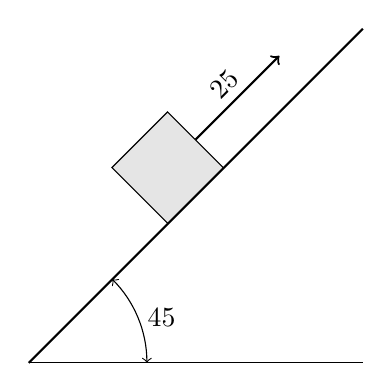
\begin{tikzpicture}
        %% incline and angle
        \draw[thick] (0,0) -- ++(45:6);
        \draw (0,0) -- ++(0:4.24);
        \draw[<->] (1.5,0) arc (0:45:1.5) node[pos=0.5,anchor=west] {\ang{45}};
        %% Block
        \node[draw,fill=white!90!black,minimum size=1cm,anchor=south,rotate=45] (A) at (45:3) {};
        \draw[thick,->] (A.east) -- ++(45:1.5) node[pos=0.5,anchor=south,rotate=45] {\SI{25}{\meter\per\second}};
    \end{tikzpicture}
    \end{center}
    If at a given time the block's velocity is \SI{+25}{\meter\per\second} in the upward direction what is the velocity of the block \SI{4.0}{\second} later?
    \begin{multicols}{3}
    \begin{choices}
        \wrongchoice{\SI{+64.2}{\meter\per\second}}
        \wrongchoice{\SI{+53.3}{\meter\per\second}}
        \wrongchoice{\SI{+28.3}{\meter\per\second}}
        \wrongchoice{\SI{+7.1}{\meter\per\second}}
      \correctchoice{\SI{-2.7}{\meter\per\second}}
    \end{choices}
    \end{multicols}
\end{question}
}

\element{aapt}{ %% Olympiad-A3
\begin{question}{olympiad-2000-q14}
    Three blocks ($m_1$, $m_2$ and $m_3$) are slid at constant velocity across a rough surface as shown below.
    \begin{center}
    \begin{tikzpicture}
        %% Ground
        \draw (-5,0) -- (2,0);
        \node[anchor=north,fill,pattern=north east lines,minimum width=7cm, minimum height=0.1cm] at (-1.5,0) {};
        %% Three Blocks
        \node[draw,minimum size=1.5cm,fill=white!90!black,anchor=south east] (A) at (0,0) {$m_1$};
        \node[draw,minimum size=1.2cm,fill=white!90!black,anchor=south east] (B) at (A.south west) {$m_2$};
        \node[draw,minimum size=1.0cm,fill=white!90!black,anchor=south east] (C) at (B.south west) {$m_3$};
        %% Force
        \draw[very thick,<-] (A.east) -- ++(0:2) node[pos=0.5,anchor=south] {$F$};
    \end{tikzpicture}
    \end{center}
    The coefficient of kinetic friction between each block and the surface is $\mu$.
    What would be the force of $m_1$ on $m_2$?
    \begin{multicols}{2}
    \begin{choices}
        \wrongchoice{$F$}
        \wrongchoice{$F -\left(m_2 - m_3\right) g\mu$}
      \correctchoice{$\left(m_2 + m_3\right) g\mu$}
        \wrongchoice{$m_1g\mu - \left(m_2 + m_3\right) g\mu$}
        \wrongchoice{$\left(m_1 + m_2 + m_3\right) g\mu$}
    \end{choices}
    \end{multicols}
\end{question}
}

\element{aapt}{ %% Olympiad-A3
\begin{question}{olympiad-2000-q17}
    %% Questions 17 and 18 refer to the situation shown in the accompanying diagram.
    Two \SI{5}{\kilo\gram} masses are attached to opposite ends of a long massless cord which passes tautly over a massless frictionless pulley.
    The upper mass is initially held at rest on a table \SI{50}{\centi\meter} from the pulley.
    The coefficient of kinetic friction between this mass and the table is \num{0.20}.
    \begin{center}
    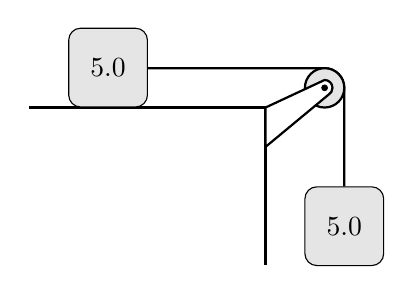
\begin{tikzpicture}
        %% Floor
        \draw[very thick] (-3,0) -- (0,0) -- (0,-2);
        %% Mass
        \node[draw,fill=white!90!black,rectangle,rounded corners=1ex,minimum size=1.0cm,anchor=south] (A) at (-2,0) {\SI{5.0}{\kilo\gram}};
        \node[draw,fill=white!90!black,rectangle,rounded corners=1ex,minimum size=1.0cm,anchor=north] (B) at (1,-1) {\SI{5.0}{\kilo\gram}};
        %% Rope and Pully
        \draw[thick] (A.south east) ++(90:0.5) -- (0.75,0.5) arc(90:0:0.25) -- (B.north);
        \draw[thick,fill=white!90!black] (0.75,0.25) circle (0.25);
        \draw[thick,fill=white] (0,0) -- (0.75,0.35) arc (90:-60:0.1) -- (0,-0.5) -- cycle;
        \draw[fill] (0.75,0.25) circle (1pt);
    \end{tikzpicture}
    \end{center}
    %% start question
    When the system is released, its resulting acceleration is closest to which of the following:
    \begin{multicols}{3}
    \begin{choices}
        \wrongchoice{\SI{9.8}{\meter\per\second\squared}}
        \wrongchoice{\SI{7.8}{\meter\per\second\squared}}
        \wrongchoice{\SI{4.9}{\meter\per\second\squared}}
      \correctchoice{\SI{3.9}{\meter\per\second\squared}}
        \wrongchoice{\SI{1.9}{\meter\per\second\squared}}
    \end{choices}
    \end{multicols}
\end{question}
}


%% PhysicsOlympiad 1999
%%----------------------------------------
\element{aapt}{ %% Olympiad-A3
\begin{question}{olympiad-1999-q02}
    Hercules and Ajax horizontally push in the same direction on a \SI{1200}{\kilo\gram} crate.
    Hercules pushes with a force of \SI{500}{\newton} and Ajax pushes with a force of \SI{300}{\newton}.
    If a frictional force provides \SI{200}{\newton} of resistance,
        what is the acceleration of the crate?
    \begin{multicols}{3}
    \begin{choices}
        \wrongchoice{\SI{1.3}{\meter\per\second\squared}}
        \wrongchoice{\SI{1.0}{\meter\per\second\squared}}
        \wrongchoice{\SI{0.87}{\meter\per\second\squared}}
        \wrongchoice{\SI{0.75}{\meter\per\second\squared}}
      \correctchoice{\SI{0.5}{\meter\per\second\squared}}
    \end{choices}
    \end{multicols}
\end{question}
}

\element{aapt}{ %% Olympiad-A3
\begin{question}{olympiad-1999-q07}
    If a net force $F$ applied to an object of mass $m$ will produce an acceleration of $a$,
        what is the mass of a second object which accelerates at $5a$ when acted upon by a net force of $2F$?
    \begin{multicols}{3}
    \begin{choices}
      \correctchoice{$\dfrac{2}{5} m$}
        \wrongchoice{$2 m$}
        \wrongchoice{$\dfrac{5}{2} m$}
        \wrongchoice{$5m$}
        \wrongchoice{$10m$}
    \end{choices}
    \end{multicols}
\end{question}
}

\element{aapt}{ %% Olympiad-A3
\begin{question}{olympiad-1999-q15}
    A \SI{4.0}{\kilo\gram} mass is attached to one end of a rope \SI{2}{\meter} long.
    If the mass is swung in a vertical circle from the free end of the rope,
        what is the tension in the rope when the mass is at its highest point if it is moving with a speed of \SI{5}{\meter\per\second}?
    \begin{multicols}{3}
    \begin{choices}
        \wrongchoice{\SI{5.4}{\newton}}
      \correctchoice{\SI{10.8}{\newton}}
        \wrongchoice{\SI{21.6}{\newton}}
        \wrongchoice{\SI{50}{\newton}}
        \wrongchoice{\SI{65.4}{\newton}}
    \end{choices}
    \end{multicols}
\end{question}
}


%% PhysicsOlympiad 1998
%%----------------------------------------
\element{aapt}{ %% Olympiad-A3
\begin{question}{olympiad-1998-q07}
    Two identical blocks of weight $W$ are placed one on top of the other as shown below.
    \begin{center}
    \begin{tikzpicture}
        %% Ground
        \draw (0,0) -- (-6,0);
        \node[anchor=north,fill,pattern=north east lines,minimum width=6cm, minimum height=0.05cm] at (-3,0) {};
        %% Wall
        \draw (0,0) -- (0,3);
        \node[anchor=west,fill,pattern=north east lines,minimum width=0.1cm, minimum height=3.2cm] at (0,+1.4) {};
        %% block
        \node[fill=white!90!black,rounded corners=1ex,minimum width=2cm,minimum height=1cm,draw,anchor=south] (B) at (-3,0) {$m$};
        \node[fill=white!90!black,rounded corners=1ex,minimum width=2cm,minimum height=1cm,draw,anchor=south] (T) at (B.north) {$m$};
        %% force
        \draw[very thick,->] (B.west) -- ++(180:1.5) node[pos=0.5,anchor=south] {$F$};
        \draw[very thick] (T.east) -- ++(0:2);
    \end{tikzpicture}
    \end{center}
    The upper block is tied to the wall.
    The lower block is pulled to the right with a force $F$.
    The coefficient of static friction between all surfaces in contact is $\mu$.
    What is the largest force $F$ that can be exerted before the lower block starts to slip?
    \begin{multicols}{3}
    \begin{choices}
        \wrongchoice{$\mu W$}
        \wrongchoice{$\dfrac{3}{2} \mu W$}
        \wrongchoice{$2 \mu W$}
        \wrongchoice{$\dfrac{5}{2} \mu W$}
      \correctchoice{$3 \mu W$}
    \end{choices}
    \end{multicols}
\end{question}
}

\element{aapt}{ %% Olympiad-A3
\begin{question}{olympiad-1998-q08}
    An object placed on an equal arm balance requires \SI{12}{\kilo\gram} to balance it.
    When placed on a spring scale, the scale reads \SI{120}{\newton}.
    Everything (balance, scale, set of masses, and the object)
        is now transported to the moon where the gravitational force is one-sixth that on Earth.
    The new readings of the balance and the spring scale (respectively) are:
    \begin{multicols}{2}
    \begin{choices}
      \correctchoice{\SI{12}{\kilo\gram}, \SI{20}{\newton}}
        \wrongchoice{\SI{12}{\kilo\gram}, \SI{120}{\newton}}
        \wrongchoice{\SI{12}{\kilo\gram}, \SI{720}{\newton}}
        \wrongchoice{\SI{2}{\kilo\gram}, \SI{20}{\newton}}
        \wrongchoice{\SI{2}{\kilo\gram}, \SI{120}{\newton}}
    \end{choices}
    \end{multicols}
\end{question}
}


%% PhysicsOlympiad 1997
%%----------------------------------------
\element{aapt}{ %% Olympiad-A3
\begin{question}{olympiad-1997-q04}
    A force $F$ is used to hold a block of mass $m$ on an incline as shown in the diagram.
    \begin{center}
    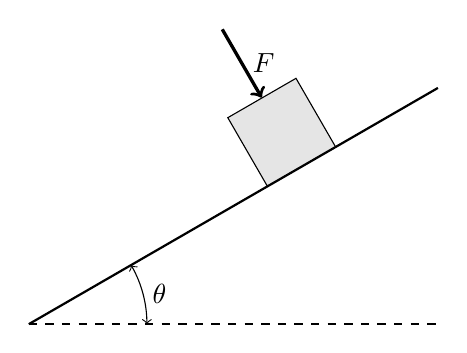
\begin{tikzpicture}
        %% incline
        \draw[thick] (0,0) -- (30:6);
        \draw[thick,dashed] (0,0) -- (0:5.196);
        \draw[<->] (1.5,0) arc (0:30:1.5) node[pos=0.5,anchor=west] {$\theta$};
        %% block
        \node[draw,anchor=south,minimum size=1cm,rotate=30,fill=white!90!black] (A) at (30:4) {};
        %% force
        \draw[very thick,<-] (A.north) -- ++(120:1) node[pos=0.5,anchor=west] {$F$};
    \end{tikzpicture}
    \end{center}
    The plane makes an angle of $\theta$ with the horizontal and $F$ is perpendicular to the plane.
    The coefficient of friction between the plane and the block is $\mu$.
    What is the minimum force, $F$, necessary to keep the block at rest?
    \begin{multicols}{2}
    \begin{choices}
        \wrongchoice{$\mu mg$}
        \wrongchoice{$mg \cos\theta$}
        \wrongchoice{$mg \sin\theta$}
        \wrongchoice{$\dfrac{mg}{\mu} \sin\theta$}
      \correctchoice{$\dfrac{mg}{\mu} \left(\sin\theta-\mu\cos\theta\right)$}
    \end{choices}
    \end{multicols}
\end{question}
}

\element{aapt}{ %% Olympiad-A3
\begin{question}{olympiad-1997-q05}
    You hold a rubber ball in your hand.
    The Newton's third law companion force to the force of gravity on the ball is the force exerted by the:
    \begin{choices}
      \correctchoice{ball on the Earth.}
        \wrongchoice{ball on the hand.}
        \wrongchoice{hand on the ball.}
        \wrongchoice{Earth on the ball.}
        \wrongchoice{Earth on your hand.}
    \end{choices}
\end{question}
}

\element{aapt}{ %% Olympiad-A3
\begin{question}{olympiad-1997-q06}
    A ball of mass $m$ is fastened to a string.
    The ball swings in a vertical circle of radius $R$ with the other end of the string held fixed.
    Neglecting air resistance,
        the difference between the string's tension at the bottom of the circle and at the top of the circle is:
    \begin{multicols}{3}
    \begin{choices}
        \wrongchoice{$mg$}
        \wrongchoice{$2 mg$}
        \wrongchoice{$4 mg$}
      \correctchoice{$6 mg$}
        \wrongchoice{$8 mg$}
    \end{choices}
    \end{multicols}
\end{question}
}


%% PhysicsOlympiad 1996
%%----------------------------------------
\element{aapt}{ %% Olympiad-A3
\begin{question}{olympiad-1996-q05}
    What is the tension $T$ in the rope if the \SI{10}{\newton} weight is moving upward with constant velocity?
    \begin{center}
    \begin{tikzpicture}
        %% Ceiling
        \node[anchor=south,fill,pattern=north east lines,minimum width=6cm, minimum height=0.05cm] at (-1,0) {};
        \draw (-4,0) -- (2,0);
        %% Rope
        \draw[very thick,->] (+1.0,0) -- (+1,-3) arc(0:-180:0.5) -- (0,-1) arc(0:135:0.5) -- ++(225:3.5) node[pos=1.0,anchor=south,yshift=0.05cm] {$T$};
        \draw[dashed] (-0.5,-0.5) ++(-0.3535,-0.1464) ++(225:3) -- ++(0:2);
        \draw[thick,<->] (-0.5,-0.5) ++(-0.3535,-0.1464) ++(225:3) ++(0:1.5) arc(0:45:1.5) node[pos=0.5,anchor=west] {\ang{45}};
        %% first pulley
        \draw[thick] (-0.5,-1) circle (0.5);
        \draw[fill=white!90!black] (-0.8,0) -- (-0.7,-1.1) arc(190:350:0.2) -- (-0.2,0) --cycle;
        \draw[fill] (-0.5,-1) circle (1.5pt);
        %% second pulley
        \draw[thick] (0.5,-3) circle (0.50);
        \draw[fill] (0.5,-3) circle (1.5pt);
        %% Masses
        \node[draw,fill=white!90!black,rectangle,rounded corners=1ex,minimum size=1.2cm,anchor=north] (B) at (0.5,-4) {\SI{10}{\newton}};
        \draw[thick] (B.north) -- (0.5,-3);
    \end{tikzpicture}
    \end{center}
    \begin{multicols}{3}
    \begin{choices}
        \wrongchoice{\SI{3.5}{\newton}}
      \correctchoice{\SI{5.0}{\newton}}
        \wrongchoice{\SI{7.1}{\newton}}
        \wrongchoice{\SI{10}{\newton}}
        \wrongchoice{\SI{14}{\newton}}
    \end{choices}
    \end{multicols}
\end{question}
}

\element{aapt}{ %% Olympiad-A3
\begin{question}{olympiad-1996-q06}
    As shown below,
        two blocks with masses $m$ and $M$ ($M>m$) are pushed by a force $F$ in both Case I and Case II.
    \begin{center}
    \begin{tikzpicture}
        %% Ground
        \node[anchor=north,fill,pattern=north east lines,minimum width=8cm, minimum height=0.05cm] at (0,0) {};
        \draw (-4,0) -- (4,0);
        %% Case I
        \begin{scope}[xshift=-1.75cm]
            \node[anchor=south east,draw,minimum size=1.4cm] (A1) at (0,0) {$M$};
            \node[anchor=south west,draw,minimum size=1.0cm] (B1) at (0,0) {$m$};
            \draw[ultra thick,<-] (A1.west) -- ++(180:1) node[pos=0.5,anchor=south] {$F$};
            \node[anchor=south] at (A1.north) {Case I};
        \end{scope}
        %% Case II
        \begin{scope}[xshift=+1.75cm]
            \node[anchor=south east,draw,minimum size=1.4cm] (A2) at (0,0) {$M$};
            \node[anchor=south west,draw,minimum size=1.0cm] (B2) at (0,0) {$m$};
            \draw[ultra thick,<-] (B2.east) -- ++(0:1) node[pos=0.5,anchor=south] {$F$};
            \node[anchor=south] at (A2.north) {Case II};
        \end{scope}
    \end{tikzpicture}
    \end{center}
    The surface is horizontal and frictionless.
    Let $R_{I}$ be the force that $m$ exerts on $M$ in case I and $R_{II}$ be the force that $m$ exerts on $M$ in case II.
    Which of the following statements is true?
    \begin{choices}
        \wrongchoice{$R_{I} = R_{II} = 0$}
        \wrongchoice{$R_{I} = R_{II}$ and is not equal to zero or $F$.}
        \wrongchoice{$R_{I} = R_{II} = F$}
      \correctchoice{$R_{I} < R_{II}$}
        \wrongchoice{$R_{I} > R_{II}$}
    \end{choices}
\end{question}
}

\element{aapt}{ %% Olympiad-A3
\begin{question}{olympiad-1996-q07}
    Two blocks, with masses \SI{17}{\kilo\gram} and \SI{15}{\kilo\gram},
        are connected by a light string that passes over a frictionless pulley of negligible mass as shown.
    \begin{center}
    \begin{tikzpicture}
        %% Ground
        \node[anchor=north,fill,pattern=north east lines,minimum width=8cm, minimum height=0.05cm] at (-1,0) {};
        \draw (-5,0) -- (3,0);
        %% Triangle
        \draw (-4,0) -- ++(45:5.657);
        \draw (+2.309,0) -- ++(120:4.619);
        %% angles
        \draw[<->] (-3,0) arc (0:45:1) node[pos=0.5,anchor=west] {\ang{45}};
        \draw[<->] (+1.309,0) arc (180:120:1) node[pos=0.5,anchor=east] {\ang{60}};
        %% pulley
        \draw[] (0,4.4) circle (0.25cm);
        \draw[fill] (0,4.4) circle (1pt);
        \draw[fill] (0,4.0) circle (1pt);
        \draw[very thick] (0,4.0) -- (0,4.4);
        \draw[thick] (0,4.65) arc(90:135:0.25) -- ++(225:2.85) node[pos=0.6,anchor=south,rotate=45] {$T_2$};
        \draw[thick] (0,4.65) arc(90:45:0.25) -- ++(-60:2.5) node[pos=0.6,anchor=south,rotate=-60] {$T_1$};
        %% left and right block
        \path (-4,0) ++(45:2.5) node[draw,rotate=45,anchor=south,minimum size=1.2cm] {\SI{17}{\kilo\gram}};
        \path (+2.309,0) -- ++(120:2) node[draw,rotate=-60,anchor=south,minimum size=1cm] {\SI{15}{\kilo\gram}};
    \end{tikzpicture}
    \end{center}
    The surfaces of the planes are frictionless.
    The blocks are released from rest.
    $T_1$ and $T_2$ are the tensions in the strings.
    Which of the following statements is correct?
    \begin{choices}
      \correctchoice{The \SI{15}{\kilo\gram} block accelerates down the plane.}
        \wrongchoice{The \SI{17}{\kilo\gram} block accelerates down the plane.}
        \wrongchoice{Both blocks remain at rest.}
        \wrongchoice{$T_1 > T_2$}
        \wrongchoice{$T_1 < T_2$}
    \end{choices}
\end{question}
}

\element{aapt}{ %% Olympiad-A3
\begin{question}{olympiad-1996-q08}
    A small block of mass $m$ starts from rest at the top of a globe of radius $R$.
    \begin{center}
    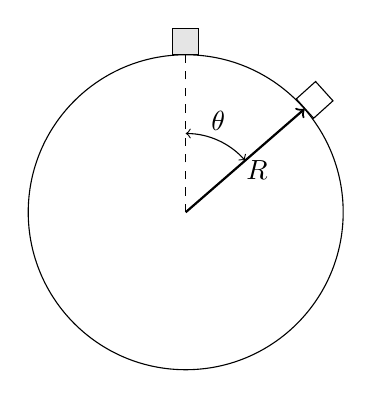
\begin{tikzpicture}
        %% globe
        \draw (0,0) circle (2cm);
        \draw[thick,->] (0,0) -- (41:2) node[anchor=north,pos=0.6] {$R$};
        \draw[dashed] (0,0) -- (90:2);
        \draw[<->] (0,1) arc(90:41:1) node[pos=0.5,anchor=south] {$\theta$};
        %% top block
        \node[anchor=south,draw,fill=white!90!black,minimum size=0.33cm] at (0,2) {};
        %% bottom block
        \node[anchor=south,draw,rotate=-48,minimum size=0.33cm] at (41:2) {};
    \end{tikzpicture}
    \end{center}
    At what angle $\theta$ does it slide off the surface of the globe?
    Assume the system is frictionless.
    \begin{multicols}{2}
    \begin{choices}
        \wrongchoice{$\theta = \ang{0}$}
        \wrongchoice{$\theta = \cos^{-1}\left(\dfrac{1}{3}\right)$}
      \correctchoice{$\theta = \cos^{-1}\left(\dfrac{2}{3}\right)$}
        \wrongchoice{$\theta = \ang{60}$}
        \wrongchoice{$\theta = \ang{90}$}
        %% added distractor ?
        %\wrongchoice{$\theta = \cos^{-1}\left(\dfrac{1}{2}\right)$}
    \end{choices}
    \end{multicols}
\end{question}
}

\element{aapt}{ %% Olympiad-A3
\begin{questionmult}{olympiad-1996-q09}
    An object with mass $m$ and initial velocity $v$ is brought to rest by a constant force $F$ acting for a time $t$ and through a distance $d$.
    %Possible expressions for the magnitude of the force $F$ are:
    Which of these give(s) the correct expression for the magnitude of the force $F$?
    \begin{multicols}{3}
    \begin{choices}
      \correctchoice{$\dfrac{mv^2}{2d}$}
      \correctchoice{$\dfrac{2md}{t^2}$}
      \correctchoice{$\dfrac{mv}{t}$}
    \end{choices}
    \end{multicols}
\end{questionmult}
}


%% PhysicsOlympiad 1995
%%----------------------------------------
\element{aapt}{ %% Olympiad-A3
\begin{question}{olympiad-1995-q03}
    Three blocks---1, 2, and 3---rest on a horizontal frictionless surface,
        as shown in the accompanying figure.
    Each block has a mass $m$, and the blocks are connected by massless strings.
    Block 3 is pulled to the right by a force $F$.
    \begin{center}
    \begin{tikzpicture}
        %% Floor
        \node[anchor=north,fill,pattern=north east lines,minimum width=8cm, minimum height=0.05cm] at (-1.5,0) {};
        \draw (-5.5,0) -- (2.5,0);
        %% Blocks
        \node[anchor=south,minimum size=1cm,draw,fill=white!90!black] (A) at (0,0) {$m$};
        \node[anchor=south,minimum size=1cm,draw,fill=white!90!black] (B) at (-2,0) {$m$};
        \node[anchor=south,minimum size=1cm,draw,fill=white!90!black] (C) at (-4,0) {$m$};
        %% Labels
        \node[anchor=south] at (A.north) {3};
        \node[anchor=south] at (B.north) {2};
        \node[anchor=south] at (C.north) {1};
        %% Strings
        \draw[thick] (A.west) -- (B.east);
        \draw[thick] (B.west) -- (C.east);
        %% Force
        \draw[thick,->] (A.east) -- ++(0:1.5cm) node[pos=0.5,anchor=south] {$F$};
    \end{tikzpicture}
    \end{center}
    The resultant force on block 2 is:
    \begin{multicols}{3}
    \begin{choices}
        \wrongchoice{zero}
      \correctchoice{$\dfrac{F}{3}$}
        \wrongchoice{$\dfrac{F}{2}$}
        \wrongchoice{$\dfrac{2F}{3}$}
        \wrongchoice{$F$}
    \end{choices}
    \end{multicols}
\end{question}
}

\element{aapt}{ %% Olympiad-A3
\begin{question}{olympiad-1995-q04}
    Which solid vector in the accompanying figures best represents the acceleration of a pendulum mass at an intermediate point in its swing?
    \begin{multicols}{2}
    \begin{choices}
        \AMCboxDimensions{down=-1cm}
        \wrongchoice{
            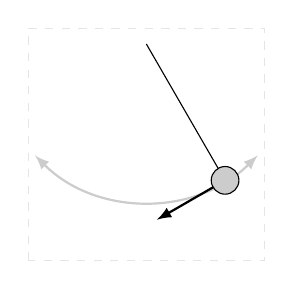
\begin{tikzpicture}
                \draw[dashed,white!90!black] (-1.5,-2.75) rectangle (1.5,0.2);
                %% string
                \draw (0,0) -- (300:2);
                %% path
                \draw[thick,white!80!black,latex-latex] (225:2) arc(225:315:2);
                %% arrows
                \draw[thick,-latex] (300:2) -- ++(210:1);
                %% bob
                \draw[fill=white!80!black] (300:2) circle (5pt);
            \end{tikzpicture}
        }
        \wrongchoice{
            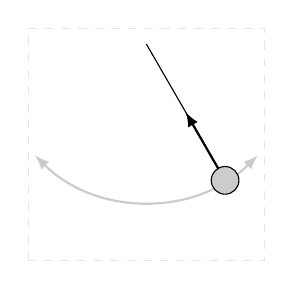
\begin{tikzpicture}
                \draw[dashed,white!90!black] (-1.5,-2.75) rectangle (1.5,0.2);
                %% string
                \draw (0,0) -- (300:2);
                %% path
                \draw[thick,white!80!black,latex-latex] (225:2) arc(225:315:2);
                %% arrows
                \draw[thick,-latex] (300:2) -- ++(120:1);
                %% bob
                \draw[fill=white!80!black] (300:2) circle (5pt);
            \end{tikzpicture}
        }
        \wrongchoice{
            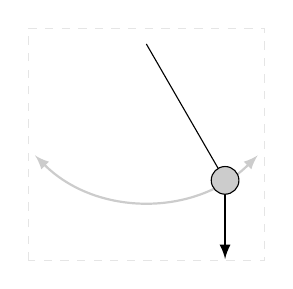
\begin{tikzpicture}
                \draw[dashed,white!90!black] (-1.5,-2.75) rectangle (1.5,0.2);
                %% string
                \draw (0,0) -- (300:2);
                %% path
                \draw[thick,white!80!black,latex-latex] (225:2) arc(225:315:2);
                %% arrows
                \draw[thick,-latex] (300:2) -- ++(270:1);
                %% bob
                \draw[fill=white!80!black] (300:2) circle (5pt);
            \end{tikzpicture}
        }
        %% ANS is D
        \correctchoice{
            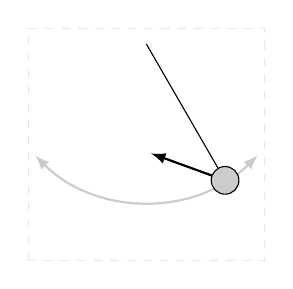
\begin{tikzpicture}
                \draw[dashed,white!90!black] (-1.5,-2.75) rectangle (1.5,0.2);
                %% string
                \draw (0,0) -- (300:2);
                %% path
                \draw[thick,white!80!black,latex-latex] (225:2) arc(225:315:2);
                %% arrows
                \draw[thick,-latex] (300:2) -- ++(160:1);
                %% bob
                \draw[fill=white!80!black] (300:2) circle (5pt);
            \end{tikzpicture}
        }
        \wrongchoice{
            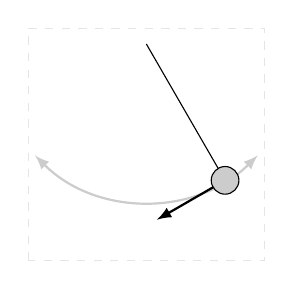
\begin{tikzpicture}
                \draw[dashed,white!90!black] (-1.5,-2.75) rectangle (1.5,0.2);
                %% string
                \draw (0,0) -- (300:2);
                %% path
                \draw[thick,white!80!black,latex-latex] (225:2) arc(225:315:2);
                %% arrows
                \draw[thick,-latex] (300:2) -- ++(210:1);
                %% bob
                \draw[fill=white!80!black] (300:2) circle (5pt);
            \end{tikzpicture}
        }
    \end{choices}
    \end{multicols}
\end{question}
}

\element{aapt}{ %% Olympiad-A3
\begin{question}{olympiad-1995-q06}
    Two identical masses $m$ are connected to a massless string which is hung over two frictionless pulleys as shown.
    \begin{center}
    \begin{tikzpicture}
        %% Ceiling
        \node[anchor=south,fill,pattern=north east lines,minimum width=8cm, minimum height=0.05cm] at (0,0) {};
        \draw (-4,0) -- (4,0);
        %% Mass Left
        \node[draw,anchor=north,minimum size=1cm,fill=white!90!black,rounded corners=0.5ex] (A) at (-2.5,-2.5) {$m$};
        %% Mass Right
        \node[draw,anchor=north,minimum size=1cm,fill=white!90!black,rounded corners=0.5ex] (B) at (+2.5,-2.5) {$m$};
        %% Rope
        \draw[very thick] (A.north) -- (-2.5,-1) arc(180:90:0.5) -- (+2,-0.5) arc(90:0:0.5) -- (B.north);
        %% Pulley Left
        \draw (-2,-1) circle (0.5cm);
        \draw[fill=white!90!black] (-2.2,0) -- (-2.1,-1.1) arc(190:350:0.1) -- (-1.8,0) -- cycle;
        \draw[fill] (-2,-1) circle (1pt);
        %% Pulley Right
        \draw (+2,-1) circle (0.5cm);
        \draw[fill=white!90!black] (+1.8,0) -- (+1.9,-1.1) arc(190:350:0.1) -- (+2.2,0) -- cycle;
        \draw[fill] (+2,-1) circle (1pt);
    \end{tikzpicture}
    \end{center}
    If everything is at rest,
        what is the tension in the cord?
    \begin{choices}
        \wrongchoice{Less than $mg$.}
      \correctchoice{Exactly $mg$.}
        \wrongchoice{More than $mg$ but less than $2mg$.}
        \wrongchoice{Exactly $2mg$.}
        \wrongchoice{More than $2mg$.}
    \end{choices}
\end{question}
}

\element{aapt}{ %% Olympiad-A3
\begin{question}{olympiad-1995-q11}
    The driver of a \SI{1000}{\kilo\gram} car tries to turn through a circle of radius \SI{100}{\meter} on an unbanked curve at a speed of \SI{10}{\meter\per\second}.
    The maximum frictional force between the tires and the slippery road is \SI{900}{\newton}.
    The car will:
    \begin{choices}
        \wrongchoice{Slide into the inside of the curve.}
        \wrongchoice{Make the turn.}
        \wrongchoice{Slow down due to the centrifugal force.}
        \wrongchoice{Make the turn only if it speeds up.}
      \correctchoice{Slide off to the outside of the curve.}
    \end{choices}
\end{question}
}


%% PhysicsOlympiad 1994
%%----------------------------------------
\element{aapt}{ %% Olympiad-A3
\begin{question}{olympiad-1994-q09}
    A horizontal force $F$, represented by the arrow in the figure below,
        is used to push a block of weight $mg$ up an inclined plane making an angle of $\theta$ with the horizontal.
    The coefficient of friction between the plane and the block is $\mu$.
    \begin{center}
    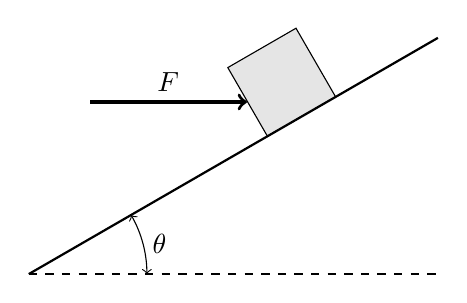
\begin{tikzpicture}
        %% incline
        \draw[thick] (0,0) -- (30:6);
        \draw[thick,dashed] (0,0) -- (0:5.196);
        \draw[<->] (1.5,0) arc (0:30:1.5) node[pos=0.5,anchor=west] {$\theta$};
        %% block
        \node[draw,anchor=south,minimum size=1cm,rotate=30,fill=white!90!black] (A) at (30:4) {};
        %% force
        \draw[very thick,<-] (A.west) -- ++(180:2) node[pos=0.5,anchor=south] {$F$};
    \end{tikzpicture}
    \end{center}
    The magnitude of the frictional force acting on the block is:
    \begin{multicols}{2}
    \begin{choices}
        \wrongchoice{$\mu mg\cos\theta$}
        \wrongchoice{$\dfrac{\mu mg}{\cos\theta}$}
      \correctchoice{$\mu\left( mg \cos\theta + F\sin\theta\right)$}
        \wrongchoice{$\mu\left(F\cos\theta - mg\sin\theta\right)$}
        \wrongchoice{$\mu F\cos\theta$}
    \end{choices}
    \end{multicols}
\end{question}
}

\element{aapt}{ %% Olympiad-A3
\begin{question}{olympiad-1994-q16}
    A simple pendulum of length $L$ and mass $m$ is attached to a moving support.
    \begin{center}
    \begin{tikzpicture}
        %% Wall
        \node[anchor=east,fill,pattern=north east lines,minimum width=0.25cm, minimum height=4.25cm] at (0,-1.85) {};
        \draw (0,0.29) rectangle (-0.29,-4);
        %% Ceiling
        \node[anchor=south,fill,pattern=north east lines,minimum width=3cm, minimum height=0.25cm] at (1.5,0) {};
        \draw (0,0) rectangle (3,0.29);
        %% Pendulum
        \draw (1.5,0) -- ++(300:3);
        \draw[fill=white!90!black] (1.5,0) ++(300:3) circle (5pt);
        %% angle
        \draw[dashed] (1.5,0) -- ++(270:3);
        \draw[<->] (1.5,0) ++(270:1.5) arc (270:300:1.5) node[pos=0.5,anchor=north] {$\theta$};
        %% length
        \draw[latex-latex] (2.5,0) -- ++(300:3) node[pos=0.5,anchor=center,fill=white,rotate=-60] {$L$};
    \end{tikzpicture}
    \end{center}
    In order for the pendulum string to make a constant angle $\theta$ with the vertical,
        the support must be moving to the:
    \begin{choices}
        \wrongchoice{right with constant acceleration $a = g\tan\theta$.}
      \correctchoice{left with constant acceleration $a = g\tan\theta$.}
        \wrongchoice{right with constant acceleration $a = g\sin\theta$.}
        \wrongchoice{right with constant velocity $v=\sqrt{Lg\tan\theta}$}
        \wrongchoice{left with constant velocity $v=\sqrt{Lg\tan\theta}$}
    \end{choices}
\end{question}
}


\endinput


